\documentclass[11pt]{article}
\usepackage[T1]{fontenc}
\usepackage[utf8]{inputenc}
\usepackage{lmodern}
\usepackage[margin=1in]{geometry}
\usepackage{amsmath,amssymb}
\usepackage{graphicx}
\graphicspath{{../results/}}
\usepackage{booktabs,xltabular,array,adjustbox,makecell}
\usepackage{enumitem}
\usepackage{url}
\usepackage[hidelinks]{hyperref}
\setlength{\parskip}{0.6em}
\setlength{\parindent}{0pt}
\setlist{itemsep=0.3em}
\renewcommand{\arraystretch}{1.15}

\title{SAE decoder geometry: where the galaxy-scale power law comes from}
\author{Ayur Pulle}
\date{November 2026}

\begin{document}
\maketitle

\begin{abstract}
The power-law eigenspectrum of SAE decoder directions reported by Li, Michaud et al. (2024) is real, but it is not a fixed property of a layer. Across the bulk of the spectrum, the decoder cloud's covariance is the activation covariance raised to a power $\gamma$, and $\gamma$ falls as L0 rises: $\gamma$ $\approx$ 1 with one active latent per token, about 0.1 lower per doubling of L0 in Gemma-2-2B. Real activations give a flatter, more width-stable cloud than a Gaussian with the same covariance. On planted data with recoverable features, $\gamma$ equals the frequency-allocation exponent and matches that theory's prediction at k = 1. In Gemma, though, the $\gamma$(k) law rides on the geometry of the dictionary's directions: in activations resynthesised from Gemma Scope's codes, it survives uniform firing frequencies and is lost on random directions.
\end{abstract}

\section{Verdict}

We asked whether the power-law eigenspectrum of SAE decoder directions is predicted by frequency-driven latent allocation (slope $\approx$ (1+$\alpha$)/(1+b), Michaud, Gorton, McGrath 2025) or is an estimator artifact. It is not an artifact. On planted data allocation produces $\gamma$ and matches its own prediction. On Gemma it fails per decoder cluster, and resynthesis places Gemma's $\gamma$(k) law in the geometry of Gemma Scope's directions, not in firing frequencies. The mid-stack peak in the top windows goes with cluster structure beyond what the covariance implies.

{\small
\begin{xltabular}{\textwidth}{>{\raggedright\arraybackslash}X>{\raggedright\arraybackslash}X>{\raggedright\arraybackslash}X}
\toprule
\textbf{Hypothesis} & \textbf{Verdict} & \textbf{Deciding evidence} \\
\midrule
\endhead
\bottomrule
\endlastfoot
Paper's finding: power-law spectrum, steepest mid-stack & Real, revised & Reproduced to 0.02\%. The exponent depends on L0, layer and rank window; the mid-stack peak is in the top $\sim$150 directions only \\
Pure estimator artifact & Not supported & Real data gives a width-stable slope and a smooth $\gamma$(L0) law; $\Sigma$-matched Gaussian and scrambled nulls do neither \\
Frequency-driven latent allocation & Not supported on Gemma; confirmed on planted data & On Gemma, latent frequencies (not the theory's feature frequencies) stay at $-$0.6 to $-$0.8 while the slope moves from $-$0.24 to $-$0.75. Per decoder cluster, mean latent frequency falls with cluster size at coarse scales (slope $-$0.6 to $-$1.5), the opposite of the prediction. Resynthesised with uniform code frequencies, Gemma's $\gamma$(k) law survives (retained 0.84). On planted circle features at k = 1, the allocation exponent is 0.33 (predicted 1/3) and $\gamma$ = 0.32 \\
The dictionary's directions carry the $\gamma$(k) law & Supported at layer 12, width 16k & Resynthesised from Gemma Scope's codes: random directions with Gemma Scope's firing statistics lose the law (retained 0.38); Gemma Scope's directions with uniform statistics keep it (0.84). Co-occurrence and the frequency--direction pairing are not needed \\
Feature splitting (near-duplicate clusters) & Ruled out & Removing near-duplicates, up to a third of latents, changes the slope by $\le$ 0.01 in 22 SAEs \\
Massive-activation tokens drive the mid-stack peak & Ruled out & Dropping the top 0.1\% or 1\% of tokens on dim 1170 changes $\gamma$ by $\le$ 0.005 \\
Inheritance from the activation covariance $\Sigma$ with exponent $\gamma$(L0) & Supported in the bulk; in the top directions only at low L0 & In $\Sigma$'s eigenbasis the decoder covariance follows $\Sigma^{\gamma}$ over ranks 101--1000 at every L0 (R$^2$ 0.94--0.99); $\gamma$ = 1.03 at k = 1 and falls about 0.1 per doubling of L0 in two SAE recipes \\
Zero-parameter law $\gamma$ = 1 $-$ ln k / ln d & Not supported & Fits at d = 2304, but with the same activations projected to d$'$ = 256 the gap between k = 8 and k = 32 is 0.01, against 0.25 predicted \\
Mismatched L0 drives the mid-stack peak & Ruled out & Measured L0 runs up to 11\% above the SAE names mid-stack; correcting for it raises the peak slightly (0.19 $\to$ 0.21) \\
\end{xltabular}}

Because $\gamma$ is defined as the ratio of the two slopes, the paper's $-$0.47 at layer 12 equals $\Sigma$'s slope there ($-$0.87) times $\gamma$ $\approx$ 0.54 by construction. The substantive claim is the matrix test in the mechanism section: the decoder cloud is aligned with $\Sigma$'s eigenbasis, and its variances follow $\Sigma$'s eigenvalues to the power $\gamma$.

\section{Reproduction}

We reproduced the paper's slopes to within 0.02\% at layers 0, 12 and 24 of Gemma-2-2B, using the computation in its released notebook.

The original computation, from \path{galaxy/PointCloudStructure_Galaxy.ipynb} in ejmichaud/feature-geometry:

\begin{itemize}
\item SAEs: \path{gemma-scope-2b-pt-res}, width 65k, one L0 per layer (73, 72 and 124 at layers 0, 12 and 24).
\item Point cloud: raw \path{W_dec} rows (65,536 $\times$ 2,304). Gemma Scope rows are already unit norm.
\item Covariance: centred, ddof = 1. Eigenvalues sorted descending.
\item Fit: least squares of log$_{10}$ eigenvalue on log$_{10}$ rank, ranks 11--150 (about 1.1 decades). The null was an N(0, 1) matrix of the same shape.
\end{itemize}

\begin{center}
\begin{adjustbox}{max width=\textwidth}
\small
\begin{tabular}{lrrrr}
\toprule
\textbf{Layer} & \textbf{Paper} & \textbf{Ours} & \textbf{R$^2$} & \textbf{\makecell[r]{Matched isotropic \\ Gaussian}} \\
\midrule
0 & $-$0.2383 & $-$0.2383 & 0.999 & $-$0.0276 \\
12 & $-$0.4684 & $-$0.4684 & 0.994 & $-$0.0276 \\
24 & $-$0.2545 & $-$0.2545 & 0.999 & $-$0.0276 \\
\bottomrule
\end{tabular}
\end{adjustbox}
\end{center}

Centring, row normalisation and dead-latent exclusion each change the slope by $\le$ 0.002. The fit window matters far more: the spectrum is curved, and moving the window one decade shifts the slope by up to 0.13. Every result below therefore reports four pre-registered windows (ranks 4--50, 11--150, 31--450, 101--1000) and counts a conclusion only if it holds in the primary window and at least two others.

\section{What sets the slope: L0, then layer, barely width}

Across 288 existing Gemma Scope SAEs, the slope is set mainly by L0 (average active latents per token), then by layer; width matters little at the top of the spectrum.

\textbf{L0.} At layer 12, slope is nearly linear in log L0 at every width from 16k to 1m: about $-$0.74 at L0 $\approx$ 12, $-$0.47 at L0 $\approx$ 72, $-$0.24 at L0 $\approx$ 445, roughly +0.10 per doubling. The paper's $-$0.47 is one point on this line.

\begin{figure}[!htbp]
\centering
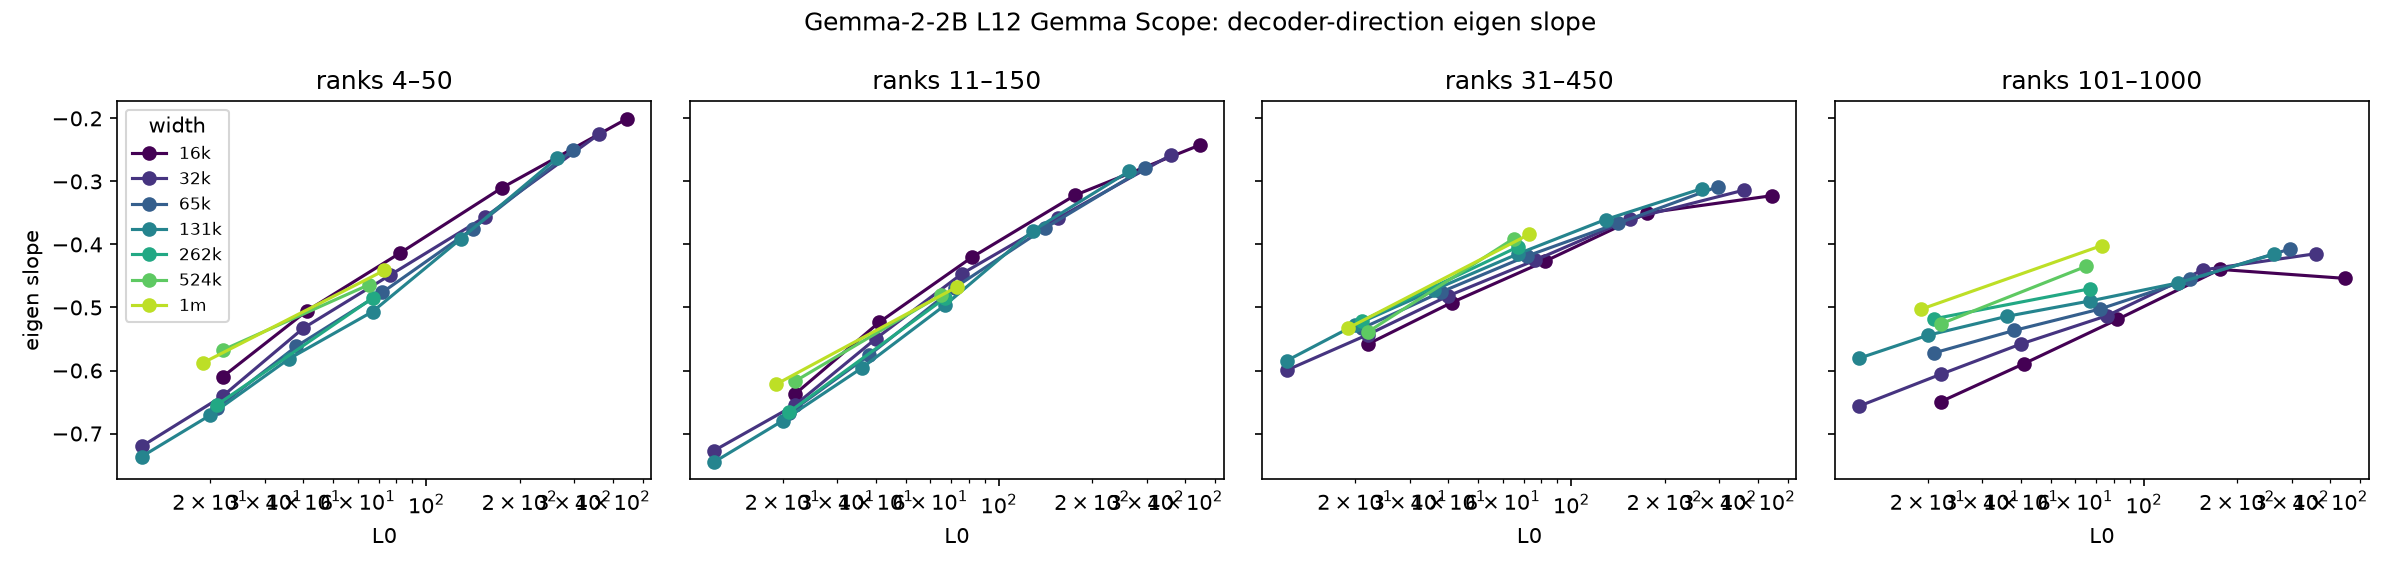
\includegraphics[width=\textwidth]{phase1/slope_vs_l0_L12.png}
\caption{Layer-12 decoder eigen slope against L0, one line per width (16k to 1m), in four rank windows.}
\end{figure}

\textbf{Width.} At matched L0, width moves the top-window slope by $\le$ 0.05 over six doublings (16k to 1m). In the deeper windows it keeps flattening with no plateau (ranks 101--1000 at L0 $\approx$ 40: $-$0.59 at 16k, $-$0.45 at 1m). "The slope converges with width" holds in only 2 of the 4 windows.

\textbf{Layer, at matched L0.} The mid-stack peak survives L0 matching in the top windows, peaking at layers 13--15 (L0 = 40: $-$0.34 at layer 0, $-$0.57 at layers 13--15, $-$0.34 at layer 23, 16k). The bulk windows show the opposite trend: steepest at layers 2--7, shallower after. The peak's amplitude shrinks with L0 (0.23 at L0 = 40, 0.06 at L0 = 140), so layer and sparsity interact. The paper's uneven L0 choice overstated the late-layer contrast by about 0.06.

\begin{figure}[!htbp]
\centering
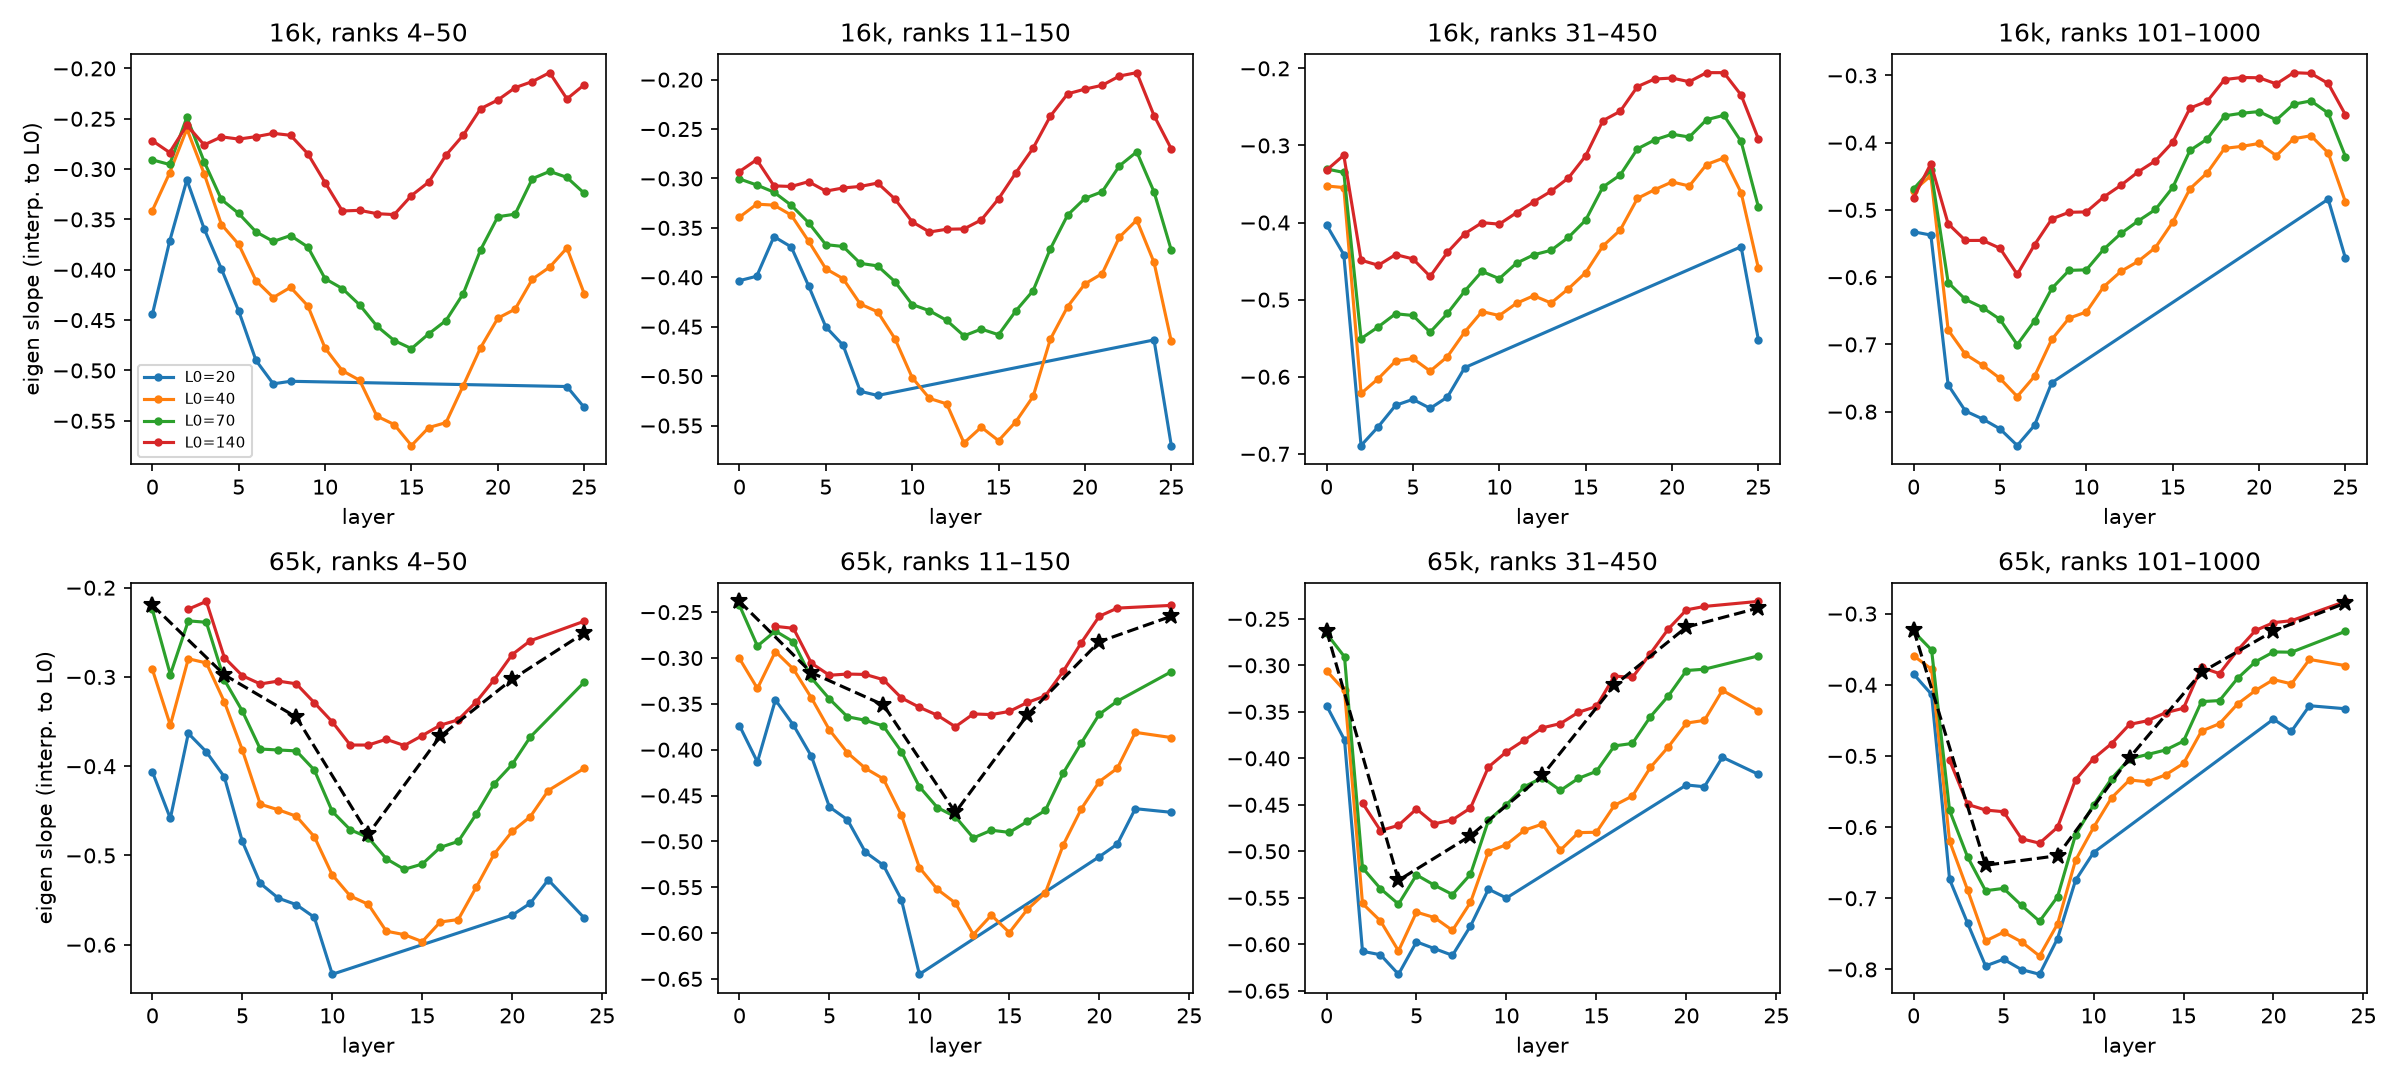
\includegraphics[width=\textwidth]{phase1/slope_vs_layer_matched_l0.png}
\caption{Decoder eigen slope against layer, interpolated to L0 = 20, 40, 70 and 140, at 16k and 65k, in four rank windows; stars mark the paper's own SAEs.}
\end{figure}

\section{Not an estimator artifact}

SAEs trained on structureless data with the same covariance do not reproduce the real geometry: real activations give a width-stable slope, while the nulls drift with width and over-concentrate the cloud.

We trained identical TopK SAEs on three inputs: real activations; a Gaussian N($\mu$, $\Sigma$) with $\mu$ and $\Sigma$ estimated from them; and scrambled activations (each coordinate permuted independently across tokens, keeping its marginal but destroying correlations). Scrambling destroys $\Sigma$'s off-diagonal structure, so scrambled runs are compared against diag($\Sigma$), not $\Sigma$. A random rotation is not a null here, since the geometry is rotation-invariant.

\textbf{Pythia-70m, layer 3} (k = 32, 15M tokens, 3 seeds). Slope, ranks 6--50:

\begin{center}
\begin{adjustbox}{max width=\textwidth}
\small
\begin{tabular}{lrrr}
\toprule
\textbf{Width} & \textbf{Real} & \textbf{\makecell[r]{Gaussian \\ N($\mu$, $\Sigma$)}} & \textbf{Scrambled} \\
\midrule
1k & $-$0.311 $\pm$ 0.007 & $-$0.299 $\pm$ 0.001 & $-$0.248 $\pm$ 0.014 \\
4k & $-$0.329 $\pm$ 0.006 & $-$0.350 $\pm$ 0.004 & $-$0.220 $\pm$ 0.013 \\
16k & $-$0.322 $\pm$ 0.007 & $-$0.391 $\pm$ 0.004 & $-$0.249 $\pm$ 0.006 \\
\bottomrule
\end{tabular}
\end{adjustbox}
\end{center}

\textbf{Gemma-2-2B, layers 3, 13, 23} (k = 40, 28.5M tokens, 16k and 65k, 3 seeds, H100). Seed-to-seed sd is $\le$ 0.015 on every value. Our real-data SAEs reach eval FVU 0.18--0.29 and give $\gamma$ = 0.43 at layer 3, against 0.41 for Gemma Scope at the same layer and L0, so a different architecture and recipe reproduces the geometry there.

\begin{itemize}
\item In the bulk (ranks 31--1000), the Gaussian and scrambled SAEs pile decoders into $\Sigma$'s top subspace ($\gamma$ 1.1--2.7). Real data spreads them out ($\gamma$ 0.29--0.81), at every layer and width. This is the largest real-vs-null difference in the project.
\item The SAE objective applied to $\Sigma$ alone does generate most of the slope's magnitude: the $\Sigma$-matched Gaussian already gives $-$0.3 to $-$0.4 in Pythia, against $-$0.13 for an isotropic Gaussian of the same shape. What real structure adds is stability, not steepness.
\end{itemize}

\textbf{Confounds checked.} The nulls do not differ because they keep fewer latents: they have 0--1 dead latents out of 16k or 65k, against 2--1,385 for real data, and every run, real or null, has $\le$ 0.4\% near-duplicate latents (cosine > 0.5). Part of the deep-window width drift is estimation: cutting 1m-wide decoders to 16k random rows moves the ranks 101--1000 slope 30--50\% of the way toward the 16k SAEs' value. The rest is geometry.

\section{The mechanism: $\Sigma$ raised to a sparsity-set power}

In $\Sigma$'s eigenbasis, the decoder cloud's variances scale as $\Sigma$'s eigenvalues to a power $\gamma$, and $\gamma$ is set by L0: $\gamma$ $\approx$ 1 at L0 = 1, falling about 0.1 per doubling. This holds across the bulk of the spectrum at every L0, and in the top directions only at low L0.

\[
\lambda_i^{\mathrm{dec}} \propto \left(\lambda_i^{\Sigma}\right)^{\gamma(L_0)}, \qquad \gamma \approx \gamma_1 - c \, \log_2 L_0
\]

\textbf{The matrix test.} Two slopes can agree by coincidence, so we tested the statement as a matrix one. We rotated the decoder covariance into $\Sigma$'s eigenbasis, checked how close to diagonal it is there, regressed its log diagonal on log $\lambda_\Sigma$, and measured the overlap of the two top eigenvector subspaces. Over ranks 101--1000 the power law holds at every L0 (R$^2$ 0.94--0.99). In the top directions it holds only up to L0 $\approx$ 85. Above that, $\gamma$ measured in the basis drops to about 0 and the overlap of the two top-10 subspaces falls to 0.09--0.13: the decoders stop tracking $\Sigma$'s leading directions. Planted data shows the same decoupling at the same ratio k/d $\approx$ 0.06--0.12. Pythia-70m's decoders ignore $\Sigma$'s top direction, which carries 36\% of the variance.

\textbf{$\Sigma$ already carries the layer profile.} We measured $\Sigma$ at all 26 Gemma layers (200k tokens). Its slope reproduces the decoder profile window for window, including the reversal: a mid-stack hump in the top windows ($-$0.72 at layer 0 to $-$0.93 at layer 14) and an early-layer peak in the bulk ($-$1.15 at layers 2--6). Decoder slope correlates moderately with $\Sigma$ slope across layers (r = +0.5 to +0.8), and $\gamma$ = decoder slope / $\Sigma$ slope averages 0.53 at L0 = 40 and 0.45 at L0 = 70 in every window.

\begin{figure}[!htbp]
\centering
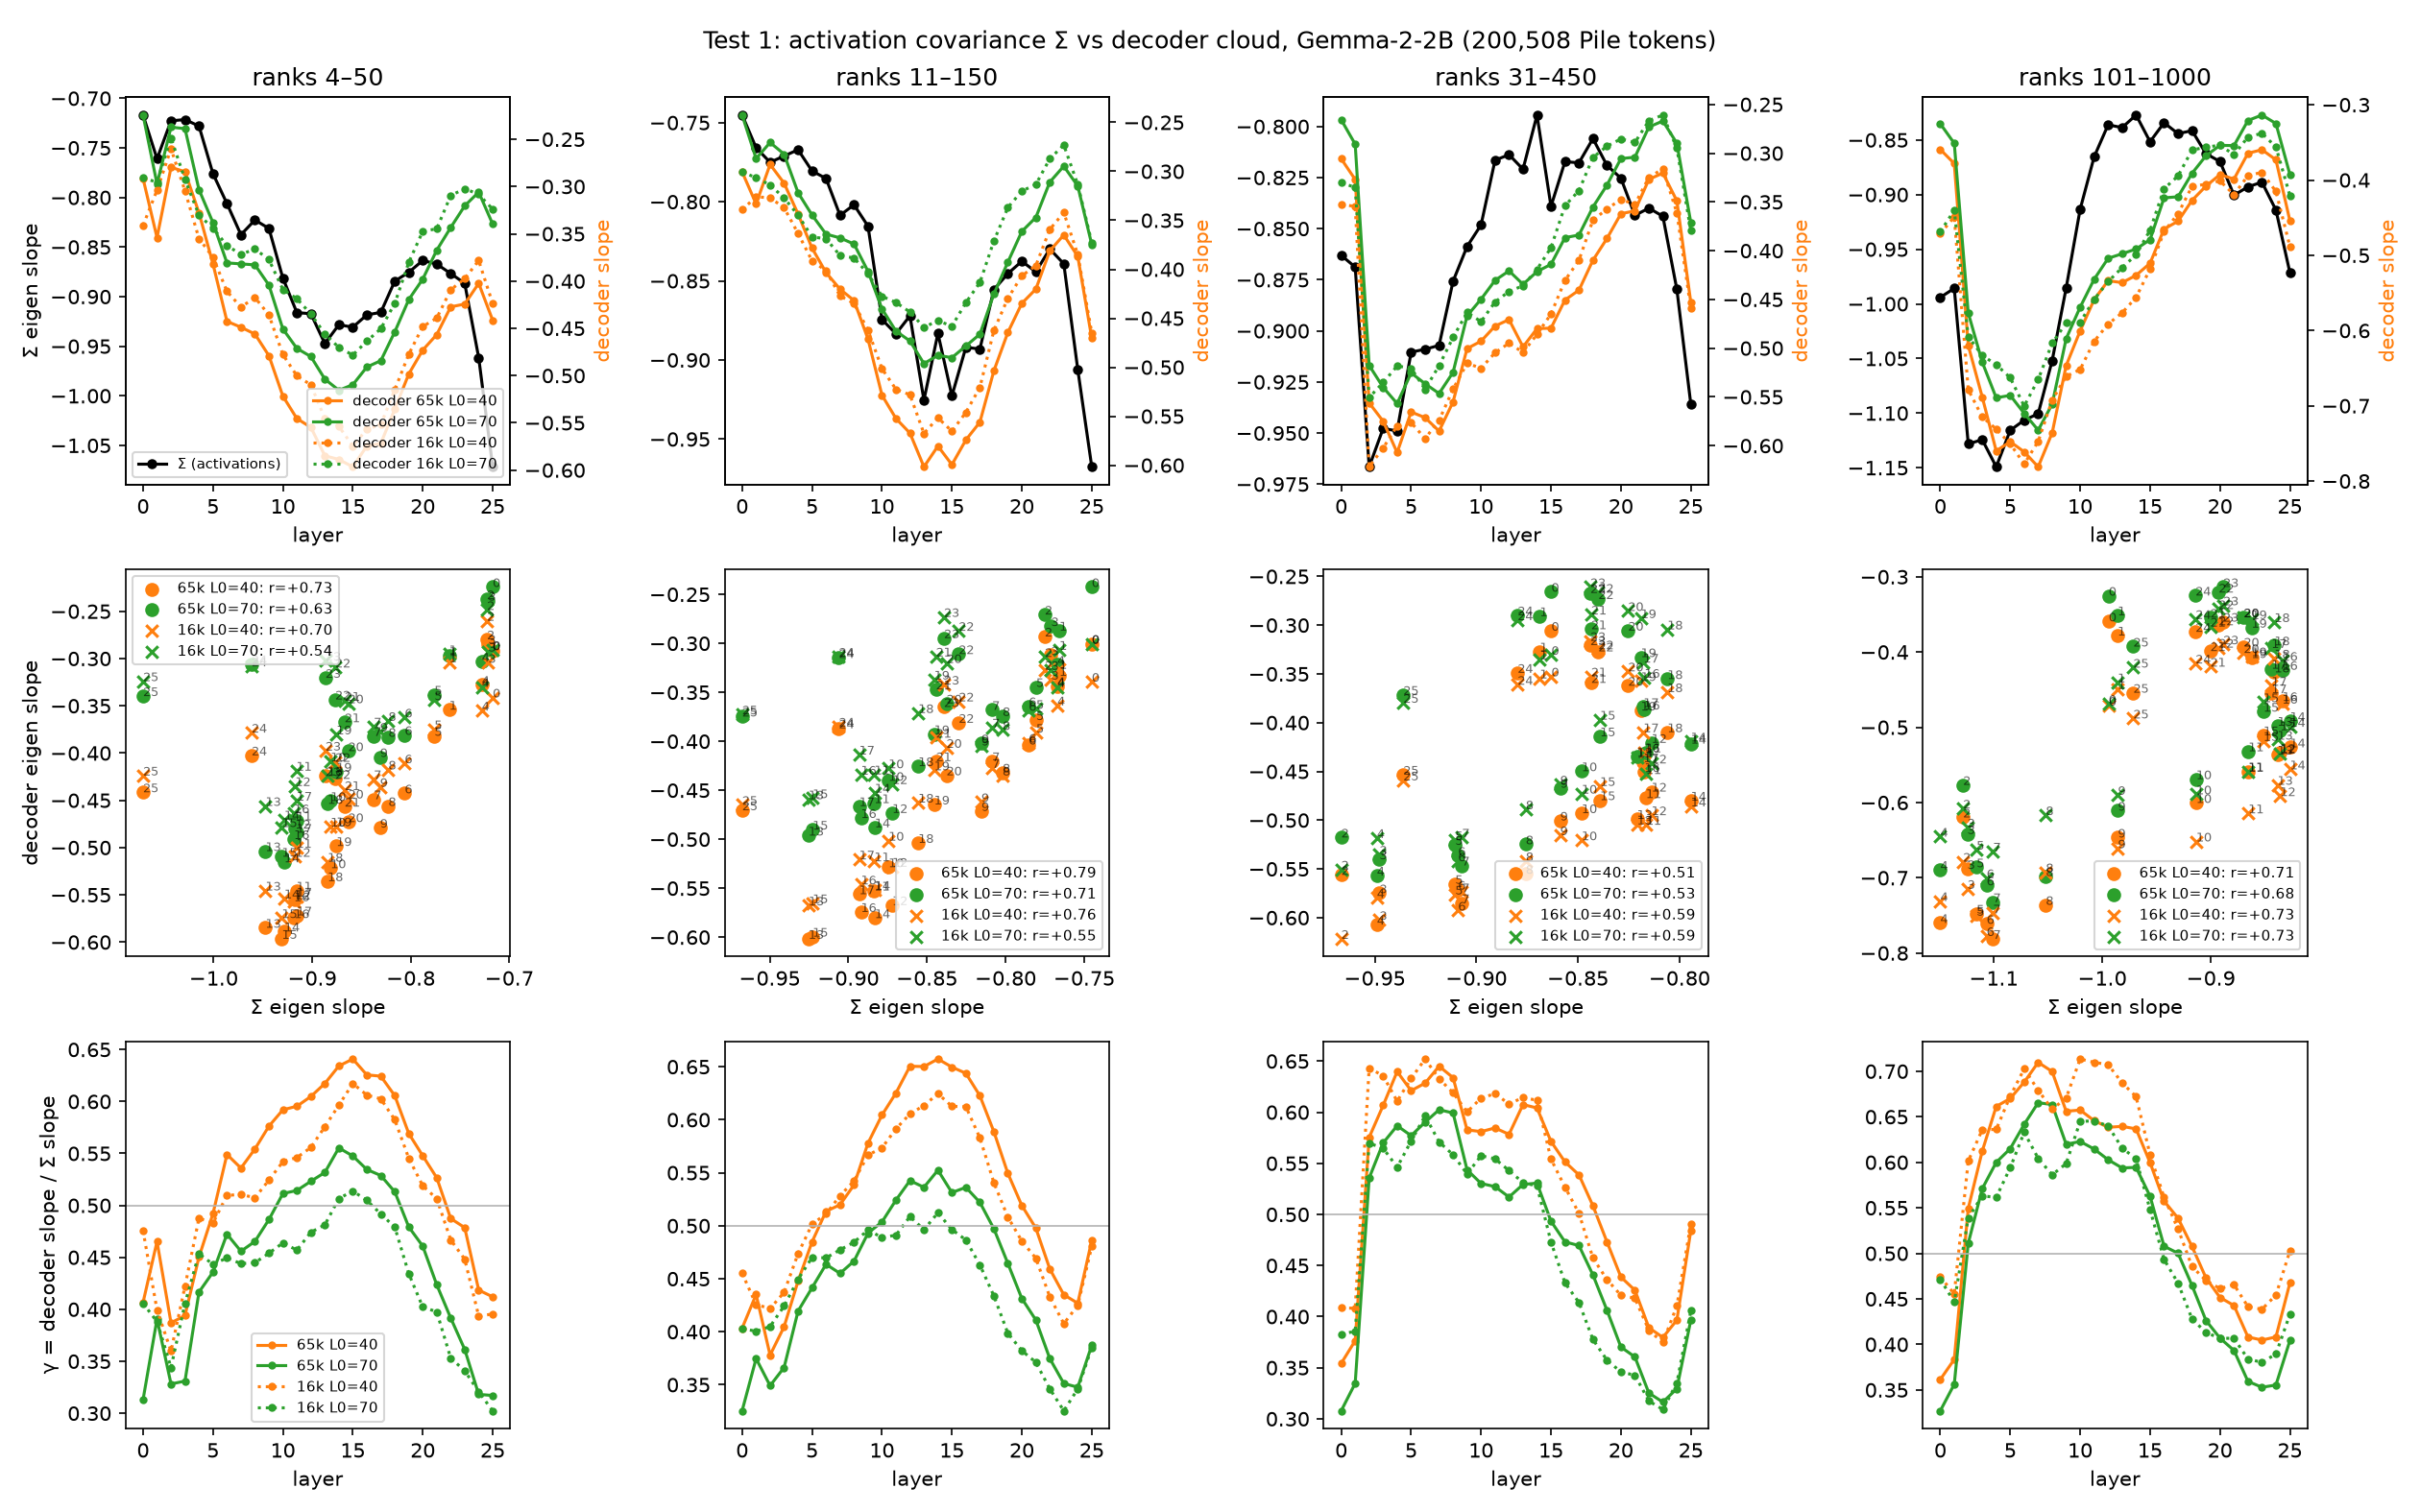
\includegraphics[width=\textwidth]{test1/sigma_vs_decoder_layers.png}
\caption{$\Sigma$ eigen slope against the decoder slope across the 26 layers (top), their scatter (middle), and $\gamma$ by layer (bottom), in four rank windows.}
\end{figure}

\textbf{At layer 12, }\textbf{$\gamma$ depends on L0 almost alone.} Across all 28 layer-12 Gemma Scope SAEs (16k to 1m), $\gamma$ = 1.245 $-$ 0.114 $\cdot$ log$_2$ L0, R$^2$ = 0.984; the width spread at fixed L0 is $\le$ 0.07 against an L0-driven range of 0.58. Across layers this does not hold: at fixed L0, $\gamma$ still varies with layer (see the mid-stack section).

\begin{figure}[!htbp]
\centering
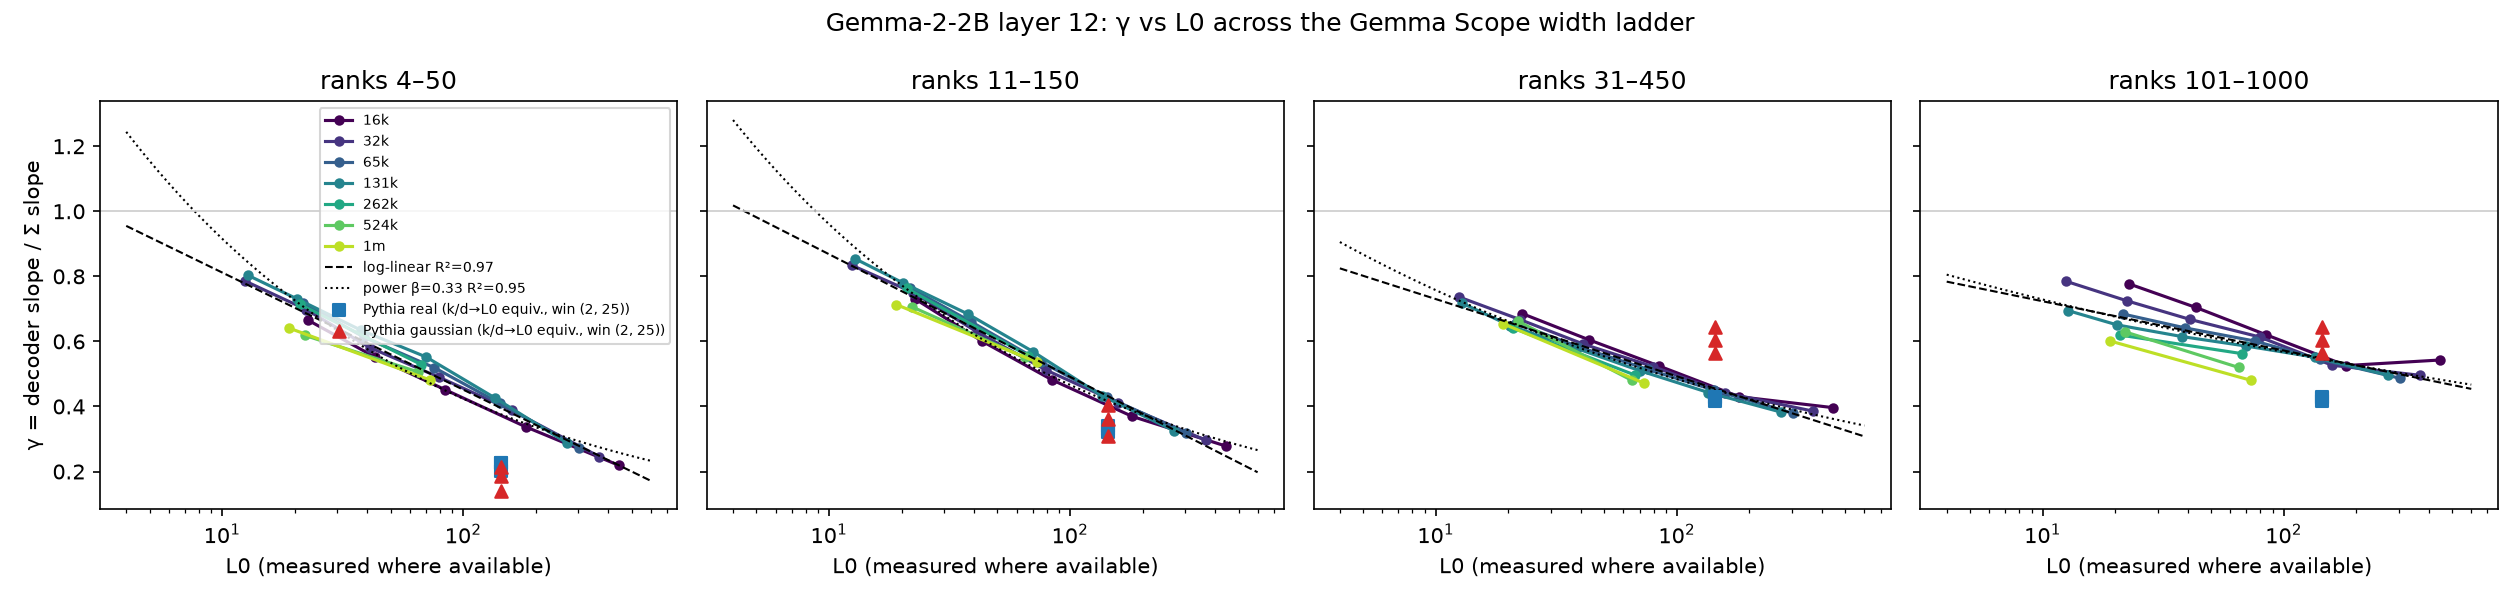
\includegraphics[width=\textwidth]{test1/gamma_l0_L12.png}
\caption{$\gamma$ against L0 at layer 12 for seven widths, with log-linear and power-law fits, in four rank windows.}
\end{figure}

\textbf{Measured directly, with our own SAEs} (layer 13, 16k, k = 1 to 128, 2 seeds). $\gamma$ in the primary window:

\begin{center}
\begin{adjustbox}{max width=\textwidth}
\small
\begin{tabular}{lrrrrrrr}
\toprule
\textbf{k (= L0)} & \textbf{1} & \textbf{2} & \textbf{4} & \textbf{8} & \textbf{16} & \textbf{40} & \textbf{128} \\
\midrule
Real & 1.034 & 0.893 & 0.824 & 0.732 & 0.665 & 0.509 & 0.354 \\
Gaussian N($\mu$, $\Sigma$) & 1.248 & 1.292 & 1.231 & 0.826 & 0.448 & 0.536 & 0.382 \\
\bottomrule
\end{tabular}
\end{adjustbox}
\end{center}

Real data follows $\gamma$ = 1.016 $-$ 0.094 $\cdot$ log$_2$ k (R$^2$ = 0.994). The functional form matches Gemma Scope's; the intercept depends on the training recipe. The Gaussian null does not follow it: it sits near 1.25 for k $\le$ 4, then drops abruptly. At k $\le$ 8 most latents die (672 of 16,384 alive at k = 1), so only the top windows are well defined there.

\textbf{An empirical fit, not a zero-parameter law.} The fit lies within 0.034 of 1 $-$ ln k / ln d with d = 2304 at every k, which suggested $\gamma$ = $\log_d(d/k)$. A dimension sweep rules that out. We projected the same layer-12 activations onto their top d$'$ principal components and trained at k = 8 and k = 32. The gap between the two k values is 0.01, 0.06, 0.13 and 0.18 at d$'$ = 256, 512, 1024 and 2304, where the law predicts 0.25, 0.22, 0.20 and 0.18. The d$'$ = 2304 control reproduces the long GPU runs (0.70 vs 0.73 at k = 8; 0.52 vs 0.51 at k = 32), so the training budget is adequate. Truncation squeezes the same features into fewer dimensions, so it is not the same as a model with smaller d; Pythia (d = 512, $\gamma$ 0.33 against 0.44 predicted) points the same way. We report the k-law as an empirical fit at d = 2304.

\textbf{A likely reason}\textbf{ $\gamma$ = 1 at k = 1.} With one latent per token, each decoder direction is a centroid of the activations it reconstructs, so the cloud samples $\Sigma$'s directions and inherits its spectrum. With more latents per token, each explains a residual left by the others, pushing decoders into lower-variance directions and flattening the cloud. This is our reading, not a derivation. Planted data adds a second, tested route to low $\gamma$: frequency-dependent allocation of latents to features.

\section{Planted features: $\gamma$ as an allocation exponent}

Synthetic activations with known features let us match latents to features and test the allocation theory directly, which is impossible on Gemma. Each token is a sparse sum of planted features with frequencies p$_i$ $\propto$ $i^{-1.5}$, plus small noise, and every dataset has a Gaussian twin with the same $\Sigma$. TopK SAEs, width 4,096, d = 256, one seed; $\gamma$ over ranks 6--50.

\textbf{Dense regime: too Gaussian.} 4,096 features, 32 active per token, directions crowded into about 37 effective dimensions. $\gamma$(k) is log-linear and close to 1 $-$ ln k / ln 256 at k = 16--64, but the Gaussian twin behaves almost identically, and at k = 4--32 at most 13\% of latents match a feature. One result carries over: the overlap between the top-10 subspaces of the decoder cloud and $\Sigma$ collapses between k/d = 0.06 and 0.12. Gemma Scope's layer-12 decoders stop tracking $\Sigma$ at the same ratio (L0 $\approx$ 150--270).

\textbf{Sparse regime: features recoverable.} 512 features, 4 active per token, random directions, so $\Sigma$'s spectrum comes from the frequencies. If feature i gets n$_i$ latents, the decoder cloud's eigenvalues scale as n$_i$ and $\gamma$ equals the exponent c in n$_i$ $\propto$ $p_i^{c.}$ For circle features (each a ring in a 2-D plane), tiling a ring with n latents leaves error $\propto$ $n^{-2}$, so the allocation law predicts c = 1/3 at k = 1 (our derivation). Point features need one latent each, so c $\approx$ 0.

{\footnotesize\setlength{\tabcolsep}{4pt}
\begin{xltabular}{\textwidth}{>{\raggedright\arraybackslash}Xrrrrrr}
\toprule
\textbf{k} & \textbf{1} & \textbf{2} & \textbf{4} & \textbf{8} & \textbf{16} & \textbf{32} \\
\midrule
\endhead
\bottomrule
\endlastfoot
Circles: allocation exponent c, top 50 features & 0.30 & 0.32 & 0.23 & 0.11 & 0.07 & $-$0.01 \\
Circles: $\gamma$ & 0.32 & 0.21 & 0.19 & 0.12 & 0.08 & 0.08 \\
Circles, Gaussian twin: $\gamma$ & 1.46* & 1.33 & 0.88 & 0.58 & 0.42 & 0.31 \\
Points: $\gamma$ & 0.30* & 0.20 & 0.16 & 0.06 & 0.04 & 0.06 \\
Points, Gaussian twin: $\gamma$ & 1.25* & 1.20 & 0.88 & 0.64 & 0.45 & 0.33 \\
\end{xltabular}}

* Fewer than 1,000 live latents.

\begin{itemize}
\item \textbf{The prediction holds at k = 1.} Over all covered circle features c = 0.334, against 1/3 predicted, and $\gamma$ is 0.32--0.35 in all three windows: $\gamma$ and the allocation exponent are the same number.
\item \textbf{Allocation flattens with k, and $\gamma$ follows.} The five most frequent circles get 11--25 latents at k = 1 and 6--9 at k $\ge$ 8. Our reading: once several latents can fire per feature, two or three combine to reconstruct any point on the ring, so tiling stops paying. In this regime the k-dependence of $\gamma$ comes from allocation.
\item \textbf{The Gaussian twin has a steeper k-law with no features at all:} $\gamma$ = 1.35--1.45 $-$ 0.22--0.25 $\cdot$ log$_2$ k, against 0.22--0.29 $-$ 0.04--0.05 $\cdot$ log$_2$ k for planted data. A k-law alone is not evidence for allocation.
\item \textbf{Gemma}\textbf{'s intercept}\textbf{ sits between the two regimes}\textbf{; its k-slope does not}\textbf{.} Its fit (1.02 $-$ 0.094 $\cdot$ log$_2$ k at layer 13) has an intercept between the sparse and dense planted data, but it falls with k about half as fast as any planted run at a similar intercept. The interpolation below tests whether density alone connects the regimes.
\item Caveats: one seed and one width. Up to 62\% of live latents in the point runs match no feature even at cosine 0.3; they fire rarely and mostly fit the noise, adding a near-isotropic floor to the cloud.
\end{itemize}

\textbf{Interpolation: density sets $\gamma$'s level, not its k-scale.} Point features, random directions, d = 256, with features per dimension and active features per token raised together. Each row is a fit $\gamma$ = A + s $\cdot$ log$_2$ k over k = 4--64 (TopK, width 4,096, one seed).

{\footnotesize\setlength{\tabcolsep}{4pt}
\begin{xltabular}{\textwidth}{>{\raggedright\arraybackslash}Xrrrrr}
\toprule
\textbf{Features, active per token} & \textbf{Planted: A} & \textbf{Planted: s} & \textbf{\makecell[r]{Gaussian \\ twin: A}} & \textbf{\makecell[r]{Gaussian \\ twin: s}} & \textbf{$-$s/A} \\
\midrule
\endhead
\bottomrule
\endlastfoot
512, 4 & 0.14 & $-$0.015 & 1.20 & $-$0.178 & 0.11*, 0.15 \\
1,024, 8 & 0.55 & $-$0.078 & 1.17 & $-$0.175 & 0.14, 0.15 \\
2,048, 16 & 1.17 & $-$0.176 & 1.39 & $-$0.210 & 0.15, 0.15 \\
4,096, 32 & 2.11 & $-$0.314 & 1.60 & $-$0.224 & 0.15, 0.14 \\
4,096, 32, crowded directions (dense regime) & 1.30 & $-$0.184 & 1.16 & $-$0.166 & 0.14, 0.14 \\
Gemma-2-2B layer 13, TopK & 1.02 & $-$0.094 &  &  & 0.09 \\
\end{xltabular}}

* Poor fit (R$^2$ 0.27): $\gamma$ is near its floor at every k.

\begin{itemize}
\item \textbf{Density moves planted $\gamma$ steadily from the allocation regime to Gaussian-like and past it.} The intercept rises 0.14 $\to$ 0.55 $\to$ 1.17 $\to$ 2.11. Planted data reaches its Gaussian twin near 2,048 features and 16 active, and overshoots it at 4,096 and 32 (2.11 vs 1.60). With crowded directions at that density, planted $\gamma$ falls back to near its twin, so crowding, not density, is what pins $\gamma$ to the Gaussian value.
\item \textbf{Every planted fit lies on one ray: s $\approx$ $-$0.15 $\cdot$ A.} Equivalently $\gamma$(k) $\approx$ A $\cdot$ (1 $-$ log$_2$ k / log$_2$ k$_0$) with k$_0$ $\approx$ $2^{6.7}$ $\approx$ 100 for every density, both direction settings, planted and Gaussian alike. Density changes the amplitude A only, never the k at which $\gamma$ would reach zero.
\item \textbf{The path misses Gemma.} Gemma's $-$s/A = 0.09 puts its k$_0$ near $2^{10.8}$ $\approx$ 1,800, off the planted ray. The blend hypothesis is half supported: density does carry $\gamma$ from the allocation value to Gaussian-like, but Gemma's slow decline with k needs a separate scale that this generator does not vary. Candidates are d, SAE width and the training recipe; d alone is doubtful, since Gemma truncated to 256 PCA dimensions had an almost flat k-dependence rather than the planted one.
\end{itemize}

\textbf{Width moves k$_0$, but only slightly.} At the density nearest Gemma's intercept (2,048 features, 16 active), we swept SAE width from 1,024 to 16,384. Planted log$_2$ k$_0$ rises about 0.25 per doubling of width, from 6.37 at 2,048 to 7.11 at 16,384, against Gemma's 10.8 at the same width. The Gaussian twin follows up to 8,192 and then levels off at 6.8. Width tilts $\gamma$(k) rather than shifting it: wider SAEs lower $\gamma$ at small k (k = 4: 0.97 $\to$ 0.67) and leave it almost unchanged at k $\ge$ 16. So the intercept and the slope shrink together. At width 8,192 the intercept matches Gemma's (1.02) but the slope is $-$0.148; at 16,384 the slope is closer ($-$0.122) but the intercept has fallen to 0.87. Most of Gemma's slow decline with k must come from something else: d, the data, or the recipe. One caveat: Gemma's fit uses ranks 11--150 and k = 1--128 at d = 2,304, so k$_0$ is not strictly comparable across the two.

\textbf{Dimension sets the amplitude; k$_0$ rises only slowly.} We then held density fixed as ratios to d (8d features, d/16 active) and swept d from 64 to 1,024, scoring $\gamma$ in a rank window that scales with d (ranks d/43 to d/5). The amplitude A rises steadily with d, from 0.44 at d = 64 to 2.08 at d = 1,024. log$_2$ k$_0$ stays at 6.5--7.0 up to d = 512 and reaches 8.05 only at d = 1,024, about +0.24 to +0.35 per doubling, driven mostly by that last point. So k$_0$ is set in absolute k, about 100--250 latents per token, not as a fraction of d.

\textbf{Putting the sweeps together:} across every planted setting, $\gamma$(k) $\approx$ A $\cdot$ (1 $-$ log$_2$ k / log$_2$ k$_0$). Density and d set A. Width and d move k$_0$ slowly. Extrapolated to Gemma's d = 2,304 and width 16k, the planted k$_0$ reaches about $2^{8.5.}$ Gemma's own k$_0$ depends on the window and the k range: $2^{8.9\textrm{--}9.2}$ in ranks 4--50, $2^{10.8}$ in ranks 11--150, and $2^{9.4\textrm{--}12.1}$ in ranks 31--450. Dimension and width therefore account for part of Gemma's slow decline with k, possibly most of it in the top window, but not robustly in the bulk. Gemma's intercept (1.02) is below the planted A at d $\ge$ 512, so a Gemma-like intercept in this family needs lower density, which moves A without moving k$_0$. One seed, one data family, and the d trend rests mostly on d = 1,024.

\textbf{At Gemma's own d and width, k$_0$ reaches Gemma's range.} We trained 60 SAEs on an A100 at d = 2,304 and width 16k. That covered three densities (2d features with d/64 active, 4d with d/32, 8d with d/16), k = 4--128, real data and Gaussian twins, and three seeds at one density. The top rank windows turned out to be unusable for this generator. Feature probabilities are capped at 0.5, and at this d the cap saturates the 25--101 most frequent features. That gives $\Sigma$ a plateau over its top ranks, with slope $-$0.1 to $-$0.4 in ranks 4--50 against Gemma's $-$0.98, so $\gamma$ there is a ratio over a near-zero denominator. In the d-scaled window (ranks 55--461), where $\Sigma$ falls with slope $-$1.0 to $-$1.3, the planted log$_2$ k$_0$ is 9.2 at the sparsest density and 15.3 at the densest. Gemma's is 13.0 in its nearest window (ranks 31--450, k = 4--128). The densest planted curve runs parallel to Gemma's, at $-$0.093 vs $-$0.083 per doubling, about 0.2--0.35 higher. So the k-scale gap seen at d = 256 is mostly a d-and-width effect. Two qualifications remain. The planted curves are less clean than Gemma's law (one density is flat until k = 64), partly because many latents die at small k with 6M training tokens. And the comparison in ranks 11--150, where Gemma's law is cleanest, needs a generator whose $\Sigma$ is a power law from rank 1. Seed spread is $\le$ 0.02 in almost every cell.

\textbf{With $\Sigma$ matched to Gemma's, the ranks 11--150 law is not reproduced.} We reran the three densities with feature magnitudes set so that feature variance falls as i$^{-1}$. That removes the plateau and gives $\Sigma$ slopes of $-$0.95, $-$0.90, $-$0.82 and $-$0.80 in ranks 4--50, 11--150, 31--450 and 55--461 (Gemma $-$0.98, $-$0.95, $-$0.75, $-$0.71). We used 12M tokens and 3 epochs, 30 SAEs in all (about 3.6 A100-hours, $\approx$ \$6.50). In ranks 11--150, real planted $\gamma$ is flat in k at every density: 0.1--0.3 at the two sparser densities and 0.36--0.46 at the densest (2 seeds, sd $\le$ 0.02). Gemma falls from 0.82 at k = 4 to 0.35 at k = 128. The best planted RMS against Gemma is 0.27. Only the densest setting in the wide windows looks like Gemma: in ranks 31--450 it falls from 0.88 at k = 8 to 0.38 at k = 128 (fit over k $\ge$ 8: A = 1.28, slope $-$0.124 per doubling, R$^2$ 0.98, log$_2$ k$_0$ = 10.3, against Gemma's 1.08, $-$0.083, 13.0). Its k = 4 point (0.44) breaks the trend. The Gaussian twin, by contrast, now has the same shape as Gemma's Gaussian twin (2.90 $\to$ 0.73 in ranks 31--450 vs Gemma's 2.20 $\to$ 0.70). So with $\Sigma$ a power law, the null carries over to planted data and the real-data curve does not. At the sparser densities planted decoders carry only a fraction of $\Sigma$'s anisotropy ($\gamma$ $\approx$ 0.1--0.3 in every window). That is what one expects when an SAE recovers random feature directions, whatever their variances. Gemma's $\gamma$ of 0.35--1.0 in the top window needs decoders that inherit much more of $\Sigma$, which points to structure the planted family lacks, such as correlated or clustered feature directions. Dead latents remain a confound: at k $\le$ 8 only 1,900--9,100 of 16,384 latents stay alive.

\textbf{Planting cluster structure raises $\gamma$ but does not give it Gemma's k-dependence.} We added clusters to the power-law generator: features in groups of 16, each at cosine $\rho$ = 0.4 or 0.6 to a random centre. This leaves $\Sigma$'s slopes within 0.03 of the unclustered version. We trained 30 SAEs at the two denser settings (k = 4--128; 2 seeds on one setting; about 4 A100-hours). The test, fixed before the run, was RMS against Gemma below 0.15 in ranks 11--150 plus a slope within 0.04 of Gemma's $-$0.094 per doubling. Every setting fails. The best RMS is 0.24, and every slope lies between $-$0.02 and +0.03 per doubling, in every window. Clusters move the level, not the shape. At $\rho$ = 0.6, mean $\gamma$ in ranks 11--150 rises from 0.16 to 0.26 at the sparser setting (4d features) and from 0.41 to 0.48 at the denser one (8d); in ranks 31--450 at 4d it rises from 0.22 to 0.44. The sparser setting at $\rho$ = 0.4 is the telling case. Its trained decoders carry Gemma's level of cluster structure beyond their covariance (excess between-cluster share +0.04 to +0.08, against Gemma's +0.054), yet its $\gamma$ stays near 0.19 and flat. At the denser setting, which has more features than latents, the decoders lose the planted clusters (excess $\approx$ 0 for k $\ge$ 16). So balanced, frequency-independent clusters do not produce Gemma's $\gamma$(k).

\section{What does not explain it}

Three candidate explanations failed direct tests on Gemma. For the first, frequency allocation, the Gemma test is underdetermined rather than decisive (see the caveat below); the planted-data section tests it directly.

{\small
\begin{xltabular}{\textwidth}{>{\raggedright\arraybackslash}X>{\raggedright\arraybackslash}X>{\raggedright\arraybackslash}X}
\toprule
\textbf{Candidate} & \textbf{Test} & \textbf{Result} \\
\midrule
\endhead
\bottomrule
\endlastfoot
Frequency-driven latent allocation (slope $\approx$ (1+$\alpha$)/(1+b)) & Firing frequencies of 22 layer-12 SAEs on 1M Pile tokens & The rank-frequency exponent stays at $-$0.6 to $-$0.8 while the eigen slope moves from $-$0.24 to $-$0.75; b would have to carry all the L0 dependence \\
Feature splitting: near-parallel latents act as large spikes & Greedy merge of latents with cosine > 0.5, then refit & Up to 34\% of latents removed (131k, L0 = 12); slope changes by $\le$ 0.010 in all 22 SAEs \\
Massive activations (residual dim 1170) & Remove latents aligned with dim 1170; separately, train without the tokens carrying its top 0.1\% or 1\% of values & Slope changes by 0.000 and $\gamma$ by $\le$ 0.005 \\
\end{xltabular}}

Two caveats. The frequency test uses latent frequencies, while the allocation theory concerns feature frequencies p$_i$, so on Gemma it leaves that theory underdetermined rather than refuted; the planted-data test measures p$_i$ directly. Near-duplicates do become more common at low L0 (2\% to 59\% of latents with a neighbour above cosine 0.5), but the merge test shows they carry none of the anisotropy.

The latent-frequency curve is not a single power law: piecewise exponents run from $-$0.4 to $-$1.2 depending on the rank window, which accounts for the disagreement in the literature ($-$0.57 to $-$0.74 in arXiv:2509.02565 against $-$1.0 to $-$1.2 in arXiv:2505.00190).

\section{The mid-stack effect}

At fixed L0, $\gamma$ itself rises toward the middle of the stack, and $\Sigma$ does not explain that rise: a Gaussian with the same $\Sigma$ moves the opposite way.

For Gemma Scope (65k, L0 = 40, ranks 11--150), $\gamma$ is about 0.40 at layers 0--3, about 0.65 at layers 12--16 and about 0.43 at layers 23--24. None of $\Sigma$'s shape statistics track this (top-eigenvalue share r = $-$0.01, participation ratio r = $-$0.33).

\textbf{Not an L0 mismatch.} We measured L0 for all 135 Gemma Scope 16k SAEs on our tokens. The names understate it mid-stack (measured over named 1.08--1.11 at layers 10--15, 0.92--1.03 elsewhere), so at matched true L0, mid-stack $\gamma$ is slightly higher than the name-based comparison showed. The peak's height above the edge layers rises from 0.19 to 0.21 (L0 = 40, primary window), and no layer moves by more than 0.023.

At equal budget, $\gamma$ of our SAEs (mean of 3 seeds, sd $\le$ 0.006):

\begin{center}
\begin{adjustbox}{max width=\textwidth}
\small
\begin{tabular}{lrrr}
\toprule
\textbf{$\gamma$, ranks 11--150} & \textbf{Layer 3} & \textbf{Layer 13} & \textbf{Layer 23} \\
\midrule
Real, 16k & 0.430 & 0.508 & 0.389 \\
Gaussian N($\mu$, $\Sigma$), 16k & 0.627 & 0.533 & 0.677 \\
Real, 65k & 0.364 & 0.387 & 0.315 \\
Gaussian N($\mu$, $\Sigma$), 65k & 0.562 & 0.485 & 0.663 \\
\bottomrule
\end{tabular}
\end{adjustbox}
\end{center}

\begin{figure}[!htbp]
\centering
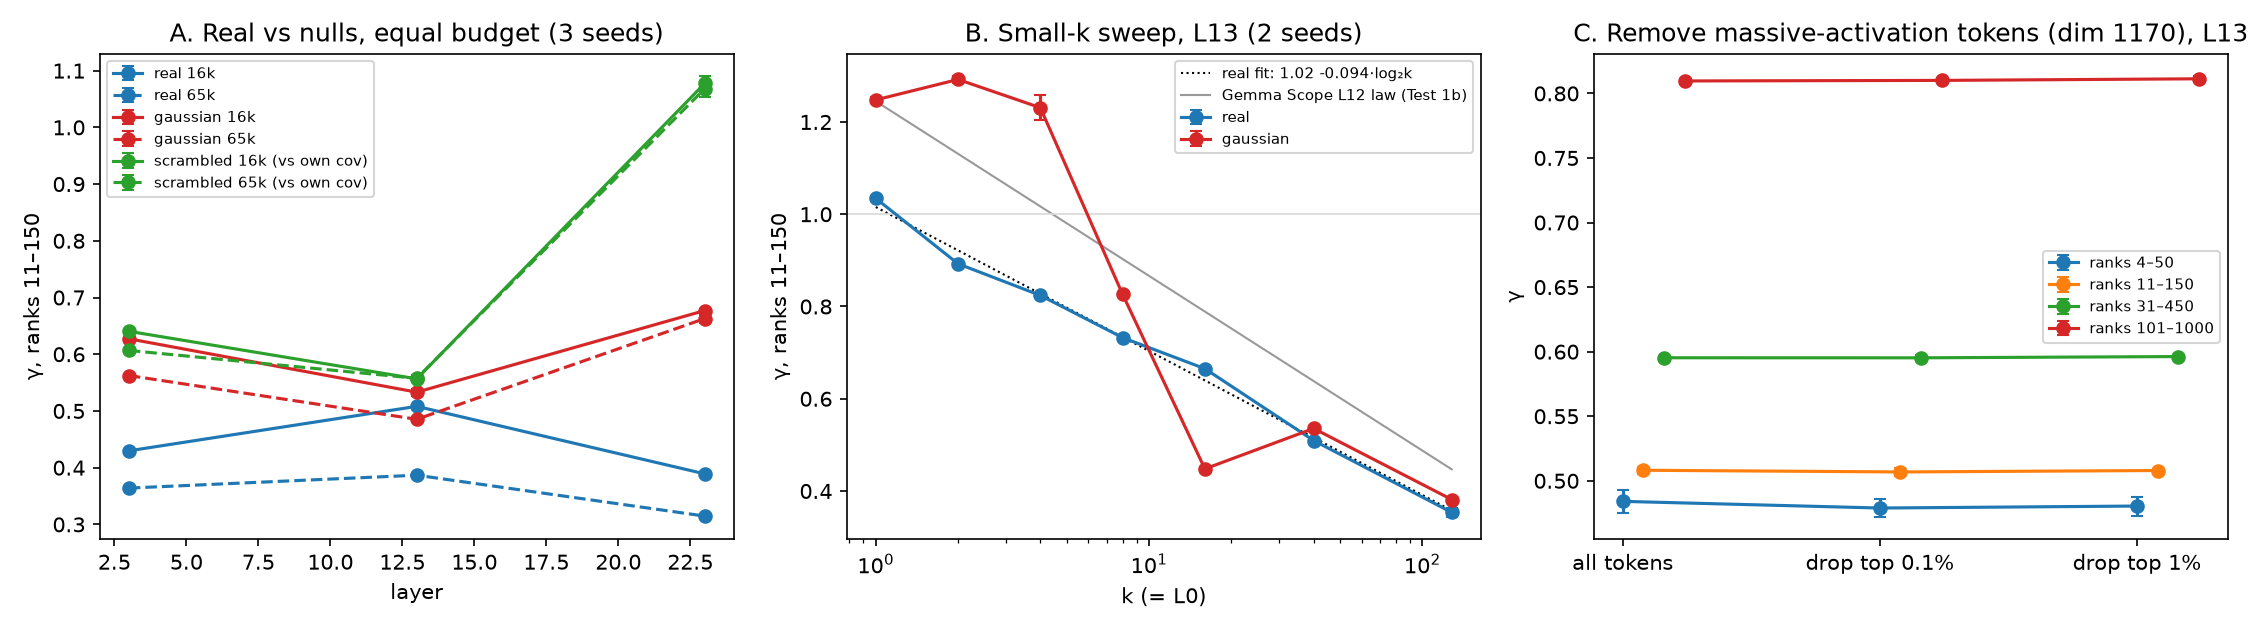
\includegraphics[width=\textwidth]{gpu/gpu_results.png}
\caption{Equal-budget results: $\gamma$ by layer for real, Gaussian and scrambled SAEs (left); $\gamma$ against k at layer 13 (centre); $\gamma$ after removing massive-activation tokens (right).}
\end{figure}

\begin{itemize}
\item The Gaussian null dips at layer 13 in every width and window. The real-minus-Gaussian gap is largest at layer 13 in all four width $\times$ window cells, the most robust form of the effect.
\item Real $\gamma$ itself peaks clearly at 16k but only weakly at 65k, and our TopK peak (0.51) is smaller than Gemma Scope's JumpReLU peak (0.65). The size of the effect depends on the SAE recipe.
\item The gap tracks the kurtosis of the massive-activation dimension across layers (r = 0.93), yet removing those tokens or the latents aligned with them changes nothing. The heavy tail marks the mid-stack regime; it does not cause the effect.
\end{itemize}

\section{Cluster structure in the decoder cloud}

Phase 3 left a gap: random planted directions give decoders much flatter than $\Sigma$, so Gemma's top-window geometry needs structure in the decoder cloud itself. We clustered Gemma Scope decoder directions (spherical k-means, Ward, average linkage, spectral) and compared each layer's cloud with a Gaussian cloud of the same covariance, unit-normalised and clustered the same way. Only the excess over that matched cloud counts as cluster structure, because a more anisotropic cloud makes any clustering look tighter. All of this ran locally on the 16k SAE nearest L0 = 70 at each of the 26 layers, plus four widths at layer 12.

\textbf{Cluster structure beyond anisotropy tracks the top-window layer profile, not the bulk.} Layer 0's cloud has no cluster structure beyond its covariance. The excess rises over layers 1--4, peaks at layers 13--15, falls through layer 23 and jumps again at layer 25, the same shape as the slope in ranks 4--50 and 11--150. Across the 26 layers, the excess between-cluster share and the excess cosine to the cluster centre correlate with the top-window slope at Spearman $-$0.87 to $-$0.91 (1,024 clusters; $-$0.78 to $-$0.90 at 256). Mid-stack clusters are also lower-dimensional than the matched cloud's: at 16 latents per cluster, their participation ratio sits up to 0.75 below it (14.1 against 14.8, maximum 15). In the deep windows (ranks 31--450, 101--1000) the excess does not track the slope (|$\rho$| $\le$ 0.45), while the matched cloud's own statistics do ($\rho$ $-$0.88 to $-$0.96). This splits Phase 1b's two layer profiles: the bulk follows anisotropy alone, and the mid-stack peak in the top windows goes with genuine cluster structure.

\textbf{Clusters carry only a minority of the top eigenvalues.} The covariance splits exactly into between-cluster and within-cluster parts. At layer 12 with 16 latents per cluster, the between-cluster part explains 27\%, 19\%, 14\% and 12\% of the eigenvalues in the four windows. A covariance-matched cloud gives 14\%, 10\%, 8\% and 7\%, and isotropic unit vectors about 8\% everywhere. Within-cluster spread still carries most of the slope (ranks 11--150: $-$0.33 within, against $-$0.42 overall). So the first-order picture of eigenvalues as cluster spikes accounts for under a third of any window. That is consistent with the near-duplicate test: the anisotropy is cloud-wide. Our own TopK SAEs at layer 12 (4,096 latents) show almost no difference between real and Gaussian-twin training data (12\% against 10\% in ranks 11--150).

\textbf{The allocation law does not hold per cluster.} Allocation predicts that the mean latent frequency in a cluster rises with the cluster's latent count (log-log slope b > 0). At layer 12, with 1M-token frequencies at widths 16k to 131k, the slope's sign depends on cluster scale. With 256 latents per cluster it is $-$0.57 to $-$1.52 (z $-$9 to $-$27 against a frequency-shuffle null): large clusters are made of rarer latents, the opposite of the prediction. Only with 16 latents per cluster at 65k and 131k is it positive (+0.21 to +0.28). Correlations are weak (|r| $\le$ 0.5), and no single b fits.

\textbf{Caveats.} Clusterings themselves are unstable: k-means against itself across seeds gives an adjusted Rand index of only 0.08--0.17, and methods agree no better. The cloud is a continuum at these scales, and only the summary statistics are robust across methods. The layer result is a correlation over 26 points on one smooth profile. The matched cloud reproduces the real spectrum within 0.02--0.05 in slope. Frequencies were measured only at layer 12.

\section{Resynthesis: the dictionary's directions carry the law}

Planted data never reproduced Gemma's $\gamma$(k) in ranks 11--150, so we built test data from Gemma itself. We encoded 12M layer-12 tokens with the Gemma Scope 65k JumpReLU SAE (L0 $\approx$ 72), resynthesised activations from its codes, and broke one ingredient at a time. Every variant trained the same TopK SAEs as the real-data baseline: width 16k, k = 4--128, 3 epochs, 500k held-out tokens. About 72 SAEs on A100s.

$\gamma$ in ranks 11--150 (mean of 2 SAE seeds for R, A, B, E and F; one seed for C and D):

{\footnotesize\setlength{\tabcolsep}{4pt}
\begin{xltabular}{\textwidth}{>{\raggedright\arraybackslash}X>{\raggedright\arraybackslash}Xrrrrrrrrr}
\toprule
\textbf{Variant} & \textbf{What it keeps} & \textbf{$\Sigma$ slope} & \textbf{k = 4} & \textbf{8} & \textbf{16} & \textbf{32} & \textbf{64} & \textbf{128} & \textbf{\makecell[r]{Slope per \\ doubling, k 8--128}} & \textbf{Retained} \\
\midrule
\endhead
\bottomrule
\endlastfoot
R: real activations & everything & $-$0.89 & 0.81 & 0.70 & 0.67 & 0.57 & 0.46 & 0.36 & $-$0.090 & --- \\
A: codes $\times$ decoder + bias & what the SAE captures & $-$0.94 & 0.78 & 0.70 & 0.67 & 0.54 & 0.44 & 0.34 & $-$0.095 & 1.00 \\
B: independent firing & per-latent frequencies and values, directions & $-$0.79 & 0.53 & 0.79 & 0.68 & 0.48 & 0.43 & 0.36 & $-$0.111 & 1.17 \\
C: decoder rows permuted & co-occurrence, directions; pairing broken & $-$0.75 & 0.67 & 0.87 & 0.59 & 0.50 & 0.42 & 0.36 & $-$0.118 & 1.24 \\
D: B and C together & frequencies, directions; unpaired & $-$0.78 & 0.55 & 0.85 & 0.66 & 0.52 & 0.45 & 0.35 & $-$0.122 & 1.28 \\
E: random directions & frequencies and values only & $-$0.84 & 0.13 & 0.23 & 0.08 & 0.07 & 0.07 & 0.06 & $-$0.036 & 0.38 \\
F: uniform frequencies, pooled values & directions only & $-$0.47 & 1.02 & 0.92 & 0.82 & 0.75 & 0.68 & 0.59 & $-$0.080 & 0.84 \\
\end{xltabular}}

Retained is a variant's slope divided by A's; above 0.75 counts as keeping the law, below 0.5 as removing it. The first run (A--D) was scored over all six k: B 0.68, C 0.95, D 0.76. Under independent firing the k = 4 point dips, so the k = 8--128 fit was fixed as primary before the second run (E, F and a second B seed). B's dip reproduces across SAE seeds ($\gamma$ 0.527 and 0.524), so it is a property of the independently fired data, not optimisation noise.

\textbf{The resynthesis is faithful.} A matches real data to RMS 0.022 across k, although its codes leave 21.5\% of the variance unexplained. The law survives losing that residual, so it lives in what the SAE captures.

\textbf{Co-occurrence and the frequency--direction pairing are not needed.} From k = 16 up, B, C and D overlap the real curve. C and D lose most of the decoder-level cluster excess, yet keep the law.

\textbf{Directions, not frequencies.} The split was read against a rule fixed before the run: if E keeps and F removes, the firing statistics carry the law; if E removes and F keeps, the dictionary's directions do. E removes (0.38) and F keeps (0.84), with per-seed slopes within 0.003 of each other. With uniform frequencies every latent stays alive at every k, and $\gamma$ still falls at close to A's rate. On random directions, $\gamma$ sits near its floor (0.06--0.23) at every k, like the planted random-direction data.

Caveats. E's "removes" is partly a floor effect: there is little $\gamma$ left to fall. F flattens $\Sigma$ ($-$0.47 against $-$0.94), so its $\gamma$ is measured against a gentler target. In ranks 4--50 and 31--450, E is partial (0.62 and 0.67) while F keeps (0.81, 0.87). There is one data draw per variant, and only layer 12 at width 16k. F tests the frequency structure of the generating codes; the trained SAE's own latent frequencies can still vary.

\section{Open questions and next steps}

The $\Sigma^{\gamma}$ law is measured but not derived. Allocation explains $\gamma$ on planted data but fails per cluster on Gemma, and resynthesis puts Gemma's $\gamma$(k) law in the dictionary's directions rather than in firing frequencies. The mid-stack top-window effect goes with cluster structure beyond anisotropy, but only as a correlation across layers, and planting balanced clusters does not reproduce Gemma's $\gamma$(k).

\begin{enumerate}
\item \textbf{Wh}\textbf{ich property of the dictionary's directions produces $\gamma$(k)?} Resynthesis puts the law in Gemma Scope's decoder directions: random directions lose it, and planted point features with Gemma's d, width and power-law $\Sigma$ never gave it, with or without balanced clusters. The next cut separates second-order from higher-order geometry: resynthesise with directions drawn from a Gaussian matching the covariance of Gemma Scope's decoder rows, then with directions shuffled within local neighbourhoods. Repeating the split at other layers, widths and L0s would show how far it generalises.
\item \textbf{Does allocation scale with manifold dimension?} The same tiling argument predicts c = m/(m+2) for m-dimensional manifold features: 1/3 for circles, 1/2 for spheres. Needs more seeds, a width ladder and m = 2 features.
\item \textbf{What makes the k-law depend on dimension?} The k-dependence vanished under PCA truncation but not in d = 256 planted data. Compare natural activations from models of different width, or planted data swept over d at fixed sparsity.
\item \textbf{Why does the mid-stack effect depend on the recipe} (JumpReLU 0.65 vs TopK 0.51 at layer 13)? Needs a few GPU-hours of JumpReLU training at matched L0.
\item \textbf{Can $\gamma$(L0) be derived?} A theory should give $\gamma$ = 1 at L0 = 1, the decline with L0, and the Gaussian's steeper decline.
\end{enumerate}

\section{Methods, code and compute}

{\small
\begin{xltabular}{\textwidth}{l>{\raggedright\arraybackslash}X}
\toprule
\textbf{Item} & \textbf{Detail} \\
\midrule
\endhead
\bottomrule
\endlastfoot
Models & Gemma-2-2B residual stream (\path{resid_post}); Pythia-70m layer 3 \\
Pretrained SAEs & Gemma Scope \path{gemma-scope-2b-pt-res}, 16k to 1m wide: decoders of 288 SAEs; encoders of all 135 16k SAEs (L0 at every layer) and of the layer-12 SAEs used for firing frequencies \\
Data & Pile (uncopyrighted subset), BOS position dropped; Gemma context 1024, Pythia 256 \\
Our SAEs & TopK with AuxK ($k_{\mathrm{aux}}$ 512), unit-norm decoder, Adam, linear LR decay over the last 20\%; inputs scaled so E$\|$x$\|^2$ = d \\
Spectrum & \path{geometry.eigen_slope}: centred covariance of decoder rows, ddof 1, least-squares log--log fit; the same function in every experiment \\
$\gamma$ & Decoder slope divided by the slope of the training data's covariance, per window \\
Windows & Ranks 4--50, 11--150 (primary), 31--450, 101--1000 for Gemma; 3--25, 6--50 (primary), 11--100 for Pythia and the d = 256 planted data \\
Planted data & synth.py: sparse sums of point or circle features with p$_i$ $\propto$ $i^{-1.5}$, d = 256, noise 0.05. Dense: 4,096 features, 32 active per token. Sparse: 512 features, 4 active, random directions. Latents matched to features at cosine > 0.7 \\
Local compute & Apple M2 Pro, 16 GB, MPS \\
GPU compute & One H100 80 GB (Runpod Secure Cloud) for 88 runs, \$50.06. A100 pods for the d = 2,304 planted, clustered, resynthesis and split runs, \$42.18 including idle and aborted pods. \$92.24 billed in total \\
\end{xltabular}}

All code, per-run JSON results and a dated research log are in the project repository (\path{notes/LOG.md}). Every result records its configuration and git commit.

\section{Sources}

\begin{itemize}
\item Li, Michaud et al. (2024), \href{https://arxiv.org/abs/2410.19750}{The Geometry of Concepts: Sparse Autoencoder Feature Structure}; code: \href{https://github.com/ejmichaud/feature-geometry}{ejmichaud/feature-geometry}
\item Michaud, Gorton, McGrath (2025), \href{https://arxiv.org/abs/2509.02565}{arXiv:2509.02565}: latent allocation model of SAE scaling
\item \href{https://arxiv.org/abs/2505.00190}{arXiv:2505.00190}: latent frequency exponents cited for comparison
\item Lieberum et al. (2024), \href{https://arxiv.org/abs/2408.05147}{Gemma Scope}: the pretrained SAEs analysed here
\item Gao et al. (2024), \href{https://arxiv.org/abs/2406.04093}{Scaling and evaluating sparse autoencoders}: the TopK SAE and AuxK loss used for our own SAEs
\end{itemize}

\end{document}
